\documentclass[12pt]{report}

%%%%%%%%%%%%%%%%%%%%%%%%%%
%%%%%% UNIT PREAMBLE %%%%% 
%%%%%%%%%%%%%%%%%%%%%%%%%%

% Basics 
\usepackage[utf8]{inputenc}
\usepackage[T1]{fontenc}
\usepackage{textcomp}
\usepackage[a4paper, left=1in, right=1in, top=1in, bottom=1in]{geometry}
\renewcommand\familydefault{\sfdefault}

\usepackage[Sonny]{fncychap}

\usepackage{amsmath,amsfonts,amsthm,amssymb,mathtools}
\usepackage[varbb]{newpxmath}
\usepackage{xfrac}
\usepackage[usenames,dvipsnames]{xcolor} % usenames, dvipsnames adds more colours
\usepackage{hhline}
\usepackage{comment}
\usepackage{tasks}
\usepackage{enumerate} 
\usepackage{enumitem} 
\usepackage{titlesec}
\usepackage[most]{tcolorbox}
\usepackage{lipsum}
\usepackage{tabularx}
\usepackage[labelfont=bf]{caption}
\usepackage{subfig}
\usepackage{pgfplots}
\usepackage{cancel} 
\usepackage{physics} 
\usepackage[bookmarks]{hyperref}
\usepackage{array}
\usepackage{float}
\usepackage{standalone}
\usepackage{graphicx}
\usepackage{forest}

% Tables 
\numberwithin{table}{section}

% Inkscape Figures
\usepackage{import}
\usepackage{xifthen}
\usepackage{pdfpages}
\usepackage{transparent}
\newcommand{\incfig}[2][1]{
    \def\svgwidth{#1\columnwidth}
    \import{../figures/}{#2.pdf_tex}
}

\pdfsuppresswarningpagegroup=1

% Chemistry
\usepackage{lewis} 
\usepackage{bohr}
\usepackage[version=4]{mhchem}

% Page setup
\hypersetup{hidelinks}
\pagenumbering{arabic}
\pagestyle{plain}
\setlength{\parindent}{0pt}

% Show subsubsections
\setcounter{tocdepth}{3}
\setcounter{secnumdepth}{3}

% Required for the Grid
\usetikzlibrary{calc}

% Section Font-Size
\titleformat{\subsubsection}
  {\normalfont\fontsize{12}{12}\bfseries}{\thesubsubsection}{1em}{}

\titleformat{\subsection}
  {\normalfont\fontsize{14}{14}\bfseries}{\thesubsection}{1em}{}

\titleformat{\section}
  {\normalfont\fontsize{16}{16}\bfseries}{\thesection}{1em}{}

% New page for each section 
\newcommand{\sectionbreak}{\clearpage}

% Section Spacing
\titlespacing{\section}{0em}{2.5em}{1em}
\titlespacing{\subsection}{0em}{2.5em}{1em}
\titlespacing{\subsubsection}{0em}{2.5em}{1em}

% TABLE COLUMN SEPARATION (USES ARRAY PACKAGE)
% \renewcommand{\arraystretch}{1.8} % changes vertical space for each cell 
% \setlength{\tabcolsep}{18pt} % changes horizontal space for each cell
% \setlength{\arrayrulewidth}{0.25mm}

% TCOLORBOX 
% \newtcolorbox[auto counter, number within=section]{definition}{colback=white,title=Example~\thetcbcounter,breakable,colframe=white,boxrule=0pt, enhanced, title style={left color=gray!60,right color=white,middle color=white},arc=0mm, titlerule=0pt, fonttitle=\bfseries\sffamily}

% Theorems 
\usepackage{thmtools}
\usepackage[framemethod=TikZ]{mdframed}

\declaretheoremstyle[
    headfont=\bfseries\sffamily\color{ProcessBlue!70!black}, bodyfont=\normalfont,
    headpunct= :,
    mdframed={
        linewidth=2pt,
        rightline=false, topline=false, bottomline=false,
        linecolor=ProcessBlue, backgroundcolor=ProcessBlue!5,
        innerbottommargin=10pt
    } ]{note}

\declaretheoremstyle[
    headfont=\bfseries\sffamily\color{NavyBlue!70!black}, 
    bodyfont=\normalfont,
    % headpunct=,
    mdframed={
        linewidth=2pt,
        rightline=false, topline=false, bottomline=false, linecolor=NavyBlue, innerbottommargin=10pt
    }
]{solution}

\declaretheoremstyle[
    headfont=\bfseries\sffamily\color{Gray!70!black}, bodyfont=\normalfont,
    % headpunct= ,
    postheadspace=\newline,
    mdframed={
        linewidth=2pt,
        rightline=false, topline=false, bottomline=false,
        linecolor=Gray, backgroundcolor=Gray!5,
        innerbottommargin=10pt
    } ]{remark}

\declaretheoremstyle[
    headfont=\bfseries\sffamily\color{Fuchsia!70!black}, bodyfont=\normalfont,
    % headpunct= ,
    mdframed={
        linewidth=2pt,
        rightline=false, topline=false, bottomline=false,
        linecolor=Fuchsia, backgroundcolor=Fuchsia!5,
        innerbottommargin=10pt
    }
]{example}

\declaretheoremstyle[
    headfont=\bfseries\sffamily\color{Fuchsia!70!black}, 
    bodyfont=\normalfont,
    % headpunct= ,
    mdframed={
        linewidth=2pt,
        rightline=false, topline=false, bottomline=false,
        linecolor=Fuchsia,
    }
]{examplesolution}

\declaretheoremstyle[
    headfont=\bfseries\sffamily\color{black!70!black}, 
    bodyfont=\normalfont,
    mdframed={
        linewidth=1pt,
        rightline=false, topline=false, bottomline=false,
        linecolor=black,
    }
]{definition}

\declaretheorem[style=solution, name=Solution, numbered=no]{solution}

\declaretheorem[style=solution, name=Derivation, numbered=no]{derivation}

\declaretheorem[style=definition, name=Definition, numberwithin=chapter]{definition}

\declaretheorem[style=note, name=Note, numbered=no]{noteswap}
\newenvironment{note}[1]{\vspace{0.5em}\begin{noteswap}[#1]}{\end{noteswap}\vspace{0.5em}}

\declaretheorem[style=remark, name=Remark, numbered=no]{remarkswap}
\newenvironment{remark}{\vspace{0.5em}\begin{remarkswap}}{\end{remarkswap}\vspace{0.5em}}

\declaretheorem[style=example, name=Example, numbered=no]{exampleswap}
% \newenvironment{example}{\vspace{0.5em}\begin{exampleswap}}{\end{exampleswap}}

\declaretheorem[style=examplesolution, name=Solution, numbered=no]{examplesolutionswap}
\newenvironment{examplesolution}{\vspace{-2em}\begin{examplesolutionswap}}{\end{examplesolutionswap}}

% Enumerate environments 
\newenvironment{2qu}
{
\begin{enumerate}[label=(\alph*)]
}
{\end{enumerate}}

\newenvironment{3qu}
{
\begin{enumerate}[label=(\roman*)]
}
{\end{enumerate}}

% Normal Environments 
\newenvironment{list0.5}
{
\begin{enumerate}
\setlength\itemsep{0.5em}
}
{\end{enumerate}}

% \titleformat{\section}{\vbox{\rule{\linewidth}{0.8pt}}\bigskip\LARGE\bfseries}{\thesection}{1em}{}

\titleformat{\section}
  {\normalfont\Large\bfseries}{\thesection}{1em}{}[{\titlerule[0.8pt]}] % horizontal line below

% thmtools Environments
\newenvironment{problems}
{
    \subsection{Problems}
    \begin{enumerate}
    \setlength\itemsep{1em}
}
{\end{enumerate}}

\newenvironment{+problems}
{
    \subsubsection{Problems}
    \begin{enumerate}
    \setlength\itemsep{1em}
}
{\end{enumerate}}

\newenvironment{example}[1]
{
    \begin{exampleswap}
        #1
    \end{exampleswap}
    \begin{examplesolution}
}
{
\end{examplesolution}}

\newenvironment{2example}[1]
{
    \begin{exampleswap}[#1]
}
{
\end{exampleswap}}

% Managing Figures
\captionsetup{width=0.8\textwidth}
\renewcommand{\thefigure}{\arabic{chapter}.\arabic{figure}}

% TABLE
% \begin{table}[h!] % delete [h!] if there are bugs

%     %%% TABLE CONFIG %%% 
%     \renewcommand{\arraystretch}{1.5} % changes vertical space for each cell 
%     \setlength{\tabcolsep}{10pt} % changes horizontal space for each cell
%     \setlength{\arrayrulewidth}{0.25mm}

%     \begin{center}
%          title of the table \
%         \vspace{0.5em}
%         \begin{tabular}{|c|c|} % use r, l, c for right, left, center. use m{3cm} for middle width of 3cm, use  b{3cm} for bottom width of 3cm, and use p{3cm} for a top width of 3cm.  
%         \hline
%          &  \ % two columns corresponding to two c's
%         \hline
%          &  \ % second row
%         \hline
%         \end{tabular}
%     \end{center}
%     \caption{}
% \end{table}

% Symbols 
\newcommand{\z}{\mathbb{Z}}

\renewcommand{\l}{\ell}

% Formatting 
\newcommand{\invis}{\vphantom{Invisible Text}}
\newcommand{\divider}{\par\noindent\rule{\textwidth}{0.5pt}\vspace{0.4em}}

% Chemistry
% \newcommand{\2ch}[2]{\ce{#1}_{(#2)}}
% \newcommand{\io}[2]{\text{#1}^{#2}} 
% \newcommand{\2io}[3]{\text{#1}^{#2}_{#3}}


\begin{document}

\section{Questions}
\begin{enumerate}
\setlength\itemsep{1em}
    \item{What is the purpose of the cell cycle?}
        \begin{solution}
            \invis
            \begin{itemize}
                \item{Sustain the processes for cell division to occur.}
                \item{Cell growth; duplication of DNA and duplication of organelles.}
                \item{Maintain regular cell function.}
            \end{itemize}
        \end{solution}

    \item{Define the term ``interphase'' and describe its purpose.}
        \begin{solution}
            It refers to the period of time in which the cell carries out its regular cell functions. The purpose of interphase is to get the cell ready to divide (growth of the cell, duplication of the cell, duplication of DNA, duplication of organelles).
        \end{solution}

    \item{
        \begin{2qu}
            \item{What is mitosis?}
                \begin{solution}
                    This is when a single parent cell divides into two new daughter cells. The parent cells and daughter cells have the same DNA.
                \end{solution}
            \item{Why is mitosis important to the cell?}
                \begin{solution}
                    \textbf{Cell reproduction}; making new cells. \textbf{Growth}; optimization of cell surface area to cell volume ratio. High surface area to volume ratio is important. A high surface area to volume ratio maintains that nutrients can enter the cell efficiently and that waste can leave the cell efficiently.
                \end{solution}
        \end{2qu}}

        \item{Define and distinguish between the following terms: chromosomes, centromere, and sister chromatids.}
            \begin{solution}
                \invis
                \begin{itemize}
                    \item{ \textbf{Chromosome}: 
                            \begin{itemize}
                                \item{Genetic material.}
                                \item{Coiled version of cellular DNA called chromatin)}
                                \item{Comprised of sister chromatids.}
                            \end{itemize}
                        }
                    \item{ \textbf{Sister chromatids}:
                            \begin{itemize}
                                \item{Identical copies of DNA which are part of the chromosomes.}
                                \item{Attached at the center with a centromere during prophase and metaphase.}
                                \item{The sister chromatids are separated in mitosis during anaphase.}
                            \end{itemize}
                        \item{ \textbf{Centromere:}
                                \begin{itemize}
                                    \item{Holds the sister chromatids together during prophase and metaphase.}
                                    \item{2 sister chromatids attached by a centromere rom the chromosome.}
                                \end{itemize}
                            }
                        }
                \end{itemize}
                \begin{figure}[H]
                \centering
                    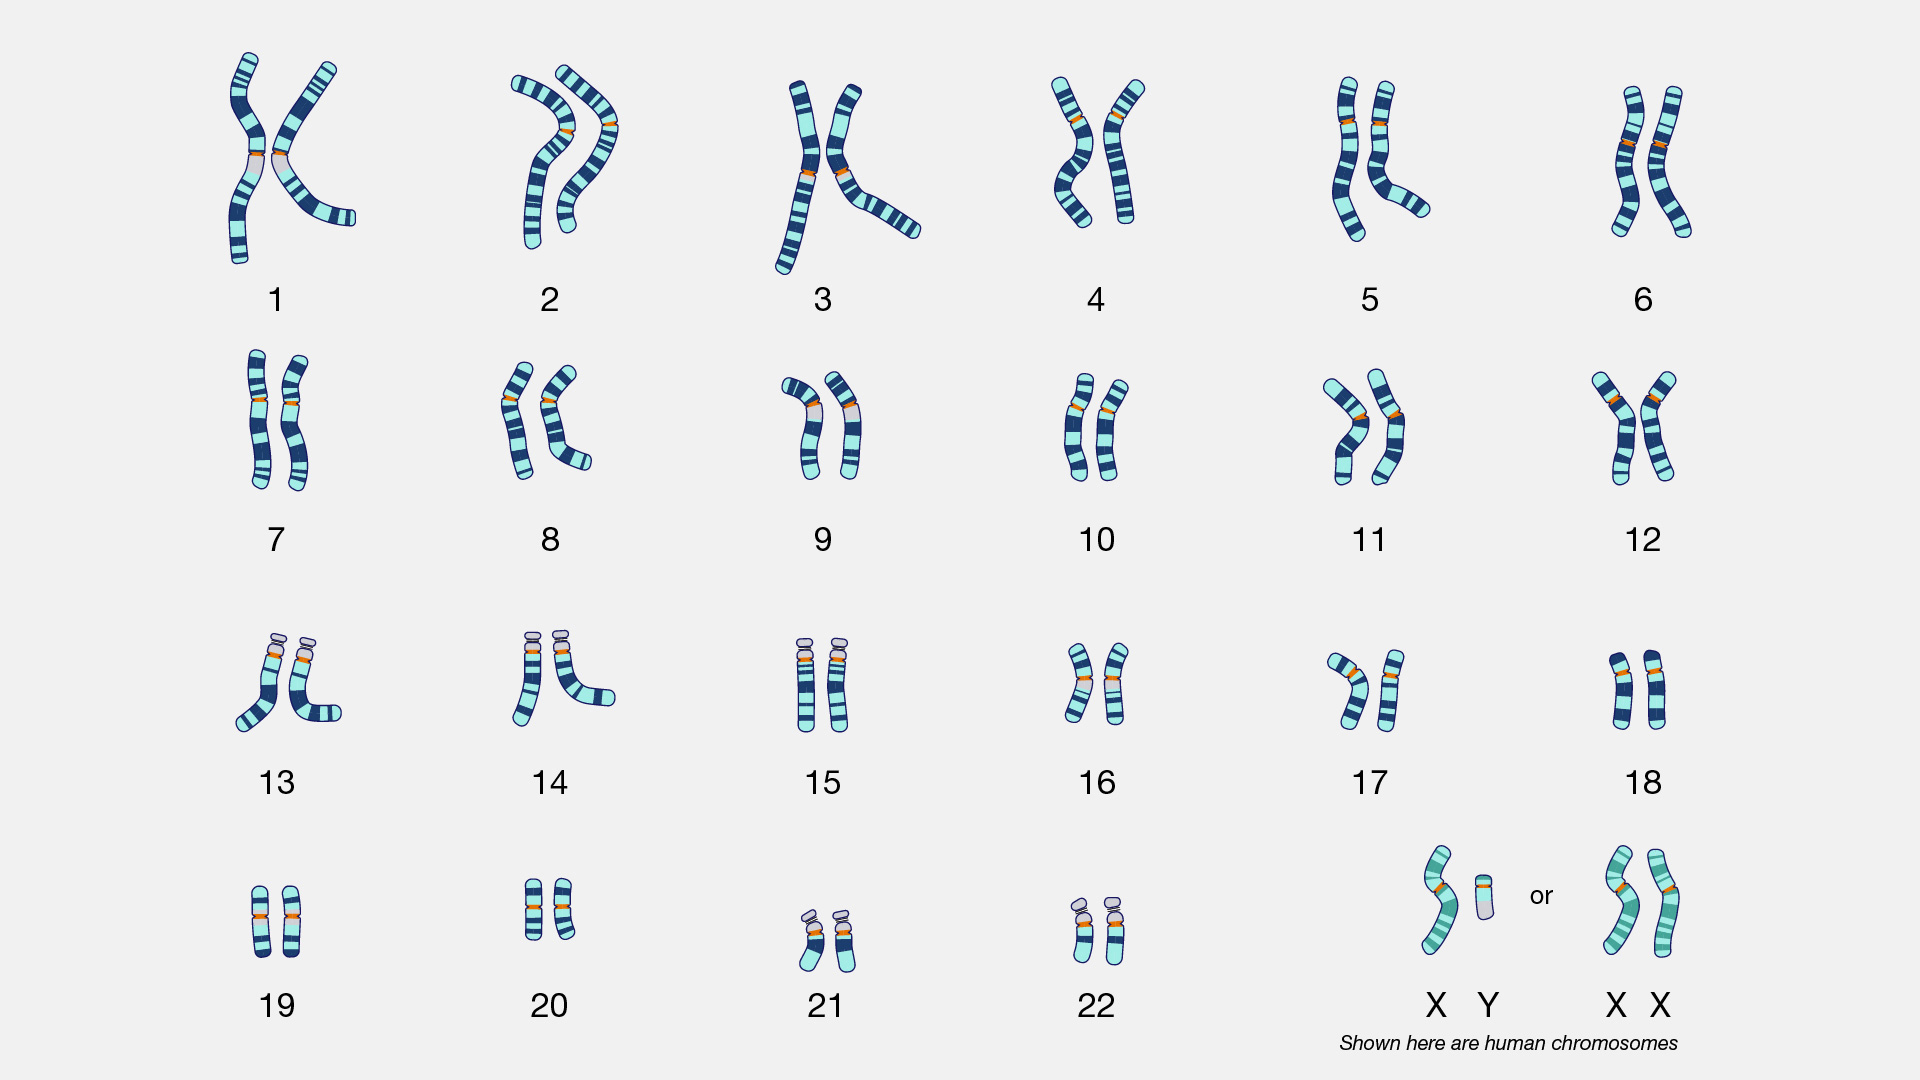
\includegraphics[width=\textwidth]{../figures/karyotype.jpg}
                    \caption{Karyotypes. In the bottom right, we see that there is XY or XX. The reason for this is because the one on the right (XY chromosome) is the male chromosome, and the one on the left (XX chromosome) is the female chromosome.}
                \end{figure}
            \end{solution}

            \item{Explain the meaning of cytokinesis.}
                \begin{solution}
                    \item{Happens after telephase. Is defined as the splitting/division of the cytoplasm. In an animal cell, this is done through the pinching of the membrane (we call this a cleavage furrow). In a plant cell, this is done through the formation of the cell plate.}
                        
                \end{solution}
\begin{figure}[ht]
    \centering
    \incfig[0.5]{animal-cell}
    \caption{Animal Cell vs Plant Cell}
    \label{fig:animal-cell}
\end{figure}
\end{enumerate}

\section{Healthy Cell Checkpoints}
\begin{definition}[Healthy Cell Checkpoints]
    A cell will not divide if 
    \begin{itemize}
        \item{Signals from surrounding cells tell the cell not to divide.}
        \item{Not enough nutrients for cell growth.}
        \item{DNA has not been replicated.}
        \item{DNA is damaged.}
    \end{itemize}
    Cell can undergo programmed cell death (apoptosis).
\end{definition}

\section{Cancer}
\begin{definition}[Cancer]
    This is a group of diseases in whcih cell grows and divides uncontrollably. See Figure \ref{fig:cancer}.
\end{definition}

This is caused by mutations to the DNA within cells which can allow rapidgrowth, fail to stop uncontrolled cell growth, or make errors when correcting DNA. Mutations arei nherited or caused by environmental factors (i.e. radiation, viruses, carcinogens, etc.).

\begin{figure}[H]
\centering
    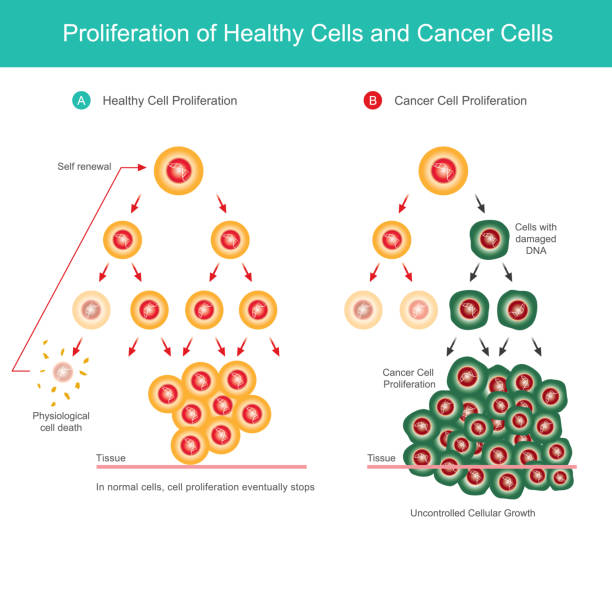
\includegraphics[width=0.75\textwidth]{../figures/cancer.jpg}
    \caption{Cancer cells stop cell division and cells are uncontrollably reproducing.}
    \label{fig:cancer}
\end{figure}

\subsection{Stages of Cancer}
% TODO
\textbf{Stage 0}: cancer cells remain in place to form a mass cells called a tumour.\\ 
\textbf{Stage 1:} small tumour has not grown deeply into nearby tissues and has not spread to lymph nodes.\\ 
\textbf{Stage 2 $\&$ 3:} larger tumours have grown deeplu into nearby tissue and may have spread to lymph nodes.\\
\textbf{Stage 4:} cancer has spread to other organs or parts of the body (metastasis).

\begin{table}[h!] % delete [h!] if there are bugs

    %%% TABLE CONFIG %%% 
    \renewcommand{\arraystretch}{1.5} % changes vertical space for each cell 
    \setlength{\tabcolsep}{10pt} % changes horizontal space for each cell
    \setlength{\arrayrulewidth}{0.25mm}

    \begin{center}
        Colorectal Cancer 5 year survival rates \\
        \vspace{0.5em}
        \begin{tabular}{|c c|} % use r, l, c for right, left, center. use m{3cm} for middle width of 3cm, use  b{3cm} for bottom width of 3cm, and use p{3cm} for a top width of 3cm.  
        \hline
        Stage & Survival Rate \\ % two columns corresponding to two c's
        \hline
        I & 94\% \\ % second row
        \hline
        II & 82\%\\ 
        \hline 
        III & 67\% \\ 
        \hline 
        IV & 11\%\\ 
        \hline
        \end{tabular}
    \end{center}
\end{table}

\newpage
\subsection{Cancer Prevention}
\textbf{Healthy choices:}
\begin{itemize}
    \item{Live smoke-free.}
    \item{Wear sunscreen and sun protection.}
    \item{Maintain a healthy body.}
    \item{Get vaccinated.}
    \item{Check your family history.}
    \item{Get screened regularly.}
\end{itemize}

\subsection{Cancer Treatment}
\begin{itemize}
    \item{ \textbf{Surgery} to physocally remove the tumour.}
    \item{ \textbf{Chemotherapy} uses chemicals and drugs to kill cancer cells; taken orally to intravenously.}
    \item{ \textbf{Radiation therapy} uses focused beams of radiation to target cancer cells.}
\end{itemize}

\end{document}
